\documentclass[a4paper]{scrartcl}

\parindent0cm

\usepackage[T1]{fontenc} 
\usepackage[utf8]{inputenc}
\usepackage[ngerman]{babel}
\usepackage{pdflscape}
\usepackage{pdfpages}
\usepackage{latexsym}
\usepackage{color}
\usepackage{booktabs,makecell,tabularx}
\usepackage{amsmath}
\usepackage{amssymb}
\usepackage{graphicx}
\usepackage[colorlinks,linkcolor = blue]{hyperref}
\usepackage{siunitx}  
\sisetup{locale = DE}
\usepackage{enumitem}

\usepackage[left=2.5cm,right=2.5cm,top=2.5cm,bottom=2cm]{geometry}

%Hintergrundbild der Titelseite
\usepackage{eso-pic}
\newcommand\BackgroundPic{%
\put(0,0){%
\parbox[b][\paperheight]{\paperwidth}{%
\vfill
\centering

\includegraphics[width=\paperwidth,height=\paperheight,%
keepaspectratio]{background.png}%
\vfill
}}}

\usepackage{showframe}

\begin{document}

\pagenumbering{Roman}

% Titelseite    
\newpage
\thispagestyle{empty}
\AddToShipoutPicture*{\BackgroundPic}

\newgeometry{top=0.6cm, bottom=2.04cm, left=2.24cm, right=2.24cm}

\begin{center}

\begin{tabular}{p{3cm}p{8cm}p{4cm}}
&\textcolor{red}{\LARGE{ }} & \vspace{-0.5cm} 
\includegraphics[height=1.4cm]{Logo_Titelseite_ohne_text.png}\\
\end{tabular}

\begin{tabular}{p{5cm}p{10.5cm}}
&\\
&
\includegraphics[height=0.9cm]{Logo_Titelseite_ohne_Symbol.png}\\
\end{tabular}

\end{center}

\vspace{7cm}

\begin{flushright}
\begin{Huge}
\textbf{Dokumentation Bachelorprojekt} \\
\end{Huge}
\vspace{2cm}
\Large{Heiko Nöldeke, Marc Bolsch, Pascal Roschkowski, Philipp Otto} \\
\vspace{0.5cm}
\LARGE{\textbf{Entwurf und Ausarbeitung eines \\ Traffic-Noise-Detector-Prototypen}}
\end{flushright}
\vspace{8cm}

\begin{center}
\begin{tabular}{lp{2cm}r}
Fakultät Technik und Informatik && Faculty of Engineering and Computer Science \\
Departement Mechatronik && Departement of Mechatronic Engineering \\
\end{tabular}
\end{center}

\newpage
\restoregeometry

\ClearShipoutPicture
\thispagestyle{empty}
\newgeometry{top=6cm, bottom=2.04cm, left=2.24cm, right=2.24cm}

\begin{center}
\Large{\textbf{Heiko Nöldeke, Marc Bolsch, Pascal Roschkowski, Philipp Otto}} \\  
\vspace{1.5cm}
\LARGE{\textbf{Traffic-Noise-Detector-Prototyp}}
\end{center}

\vspace{14cm}

\begin{tabular}{l}
Bachelorprojekt eingereicht im Rahmen der Bachelorprüfung \\
\\
im Studiengang Mechatronik \\
am Departement Fahrzeugtechnik und Flugzeugbau \\
der Fakultät Technik und Informatik \\
der Hochschule für Angewandte Wissenschaften Hamburg\\
\\
Erstprüfer: Prof. Dr. Rasmus Rettig\\
\\
Abgabedatum: \today
\end{tabular}

\newpage
\restoregeometry
\tableofcontents
\thispagestyle{empty}
\newpage

\pagenumbering{arabic}

\section{Vorwort}

Im Rahmen eines Bachelors Projekts im Fachbereich Mechatronik an der HAW Hamburg, ist eine kleine Gruppe Studierender dazu beauftragt, eine praxisnahe Aufgabe zu lösen. Dazu gehört der Prozess der Produktentwicklung, aber auch die Erschaffung eines Prototypen. Diese Dokumentation dient dazu, die Arbeitsschritte und eine Produktbeschreibung festzuhalten. Auf der Basis der Arbeit von Maximilian Welz führen die vier genannten Autoren unter Leitung von Herrn Prof. Dr. Rasmus Rettig eine Anpassung des <Bezeichnung> an die neue Aufgabenstellung an.
\newpage

\section{Git}
\begin{tabular}{|l|l|}
\hline
Git-Befehl & Auswirkung\\
\hline
\hline
git clone plus Link & Git-Verzeichnis auf PC klonen\\
\hline
git pull & aktuellen Stand vom Server holen\\
\hline
git status & Informationen über den aktuellen Stand\\
\hline
git add & geänderte Dateien hinzufügen mit Dateiname\\
\hline
git add . & alle geänderten Dateien hinzufügen\\ 
\hline
git commit -m \glqq Kommentar\grqq & Commit erstellen\\
\hline
git push & auf den Sever schieben\\
\hline
\end{tabular}

\newpage

\section{Zusammenfassung der Aufgabenstellung}

\begin{tabular}{|p{15cm}|}
\hline
\textbf{Project Charter:} Traffic-Noise-Detector (Lärmblitzer), Bachelor Project - Hr. Otto, Hr. Nöldeke, Hr. Bolsch, Hr. Roschkowski\\
\hline
\textbf{Mission:} Aufbau eines Prototypen zur Erkennung und Lokalisierung von Fahrzeigen mit (zu) hoher Lärm Emission (z. B. \url{https://www.auto-motor-und-sport.de/verkehr/laerm-blitzer-in-europa-fallen-gegen-auto-poser/}).\\
\hline
\textbf{Deliverables (incl. timing):}
\begin{itemize}
\item Anforderungsentwicklung (Mechanisch, Akustisch, Elektrisch, Algorithmisch)
\item Systematische Auswahl / ggf. Kombination oder Weiterentwicklung
\item Realisierung
\item Test und Bewertung der Eignung
\item Überarbeitung basierend auf den Testergebnissen [T0+6 Wochen]
\item Abschlussintegration, Demonstration/Vortag und Dokumentation [T0+12 Wochen]
\end{itemize}\\
\hline
\textbf{Expected Scope / Approach / Activities:}
\begin{itemize}
\item Einarbeitung in das Messsystem und die Programmierumgebung
\item Einarbeitung in den Stand der Technik von Algorithmen zur Erkennung und Lokalisierung akustischer Signale
\item Zielgerichtete Auswahl, Weiterentwicklung / Kombination im Hinblick auf genutzte Hardware sowie die Erkennung mit einer hohen Erkennungsrate
\end{itemize}\\
\hline
\textbf{Strategic alignment factors:}
\newline
Integration in dei Arbeitsgruppe Urban Mobility Lab mit den laufenden Arbeiten\\
\hline
\textbf{Timeframe/Duration:}
\begin{itemize}
\item Start 1.10.2020 (Vorbereitung
\item Abschluss 30.3.2021 (gerne früher)
\end{itemize}\\
\hline
\textbf{Team Resources:}
\newline
Nutzung Labor Stiftstraße 69 Raum 109 mit der dort verfügbaren Infrastruktur (Elektronikentwicklung, Software Entwicklung, Server, Löteinrichtung; Kamera, Testfahrzeug, Rechner)\\
\hline
\textbf{Team Process:}
\begin{itemize}
\item Reglmäßige Reviews (14 tägig)
\item Optional: Teilnahme am Teammeeting
\end{itemize}\\
\hline
\end{tabular}

\newpage

\section{Brainstorming}

Im Rahmen des Projekts wird anhand des stationären Blitzers am Anckelmannsplatz (Hamburg, Deutschland) eine mögliche Arbeitsumgebung erarbeitet.

\begin{figure}[h]
\centering
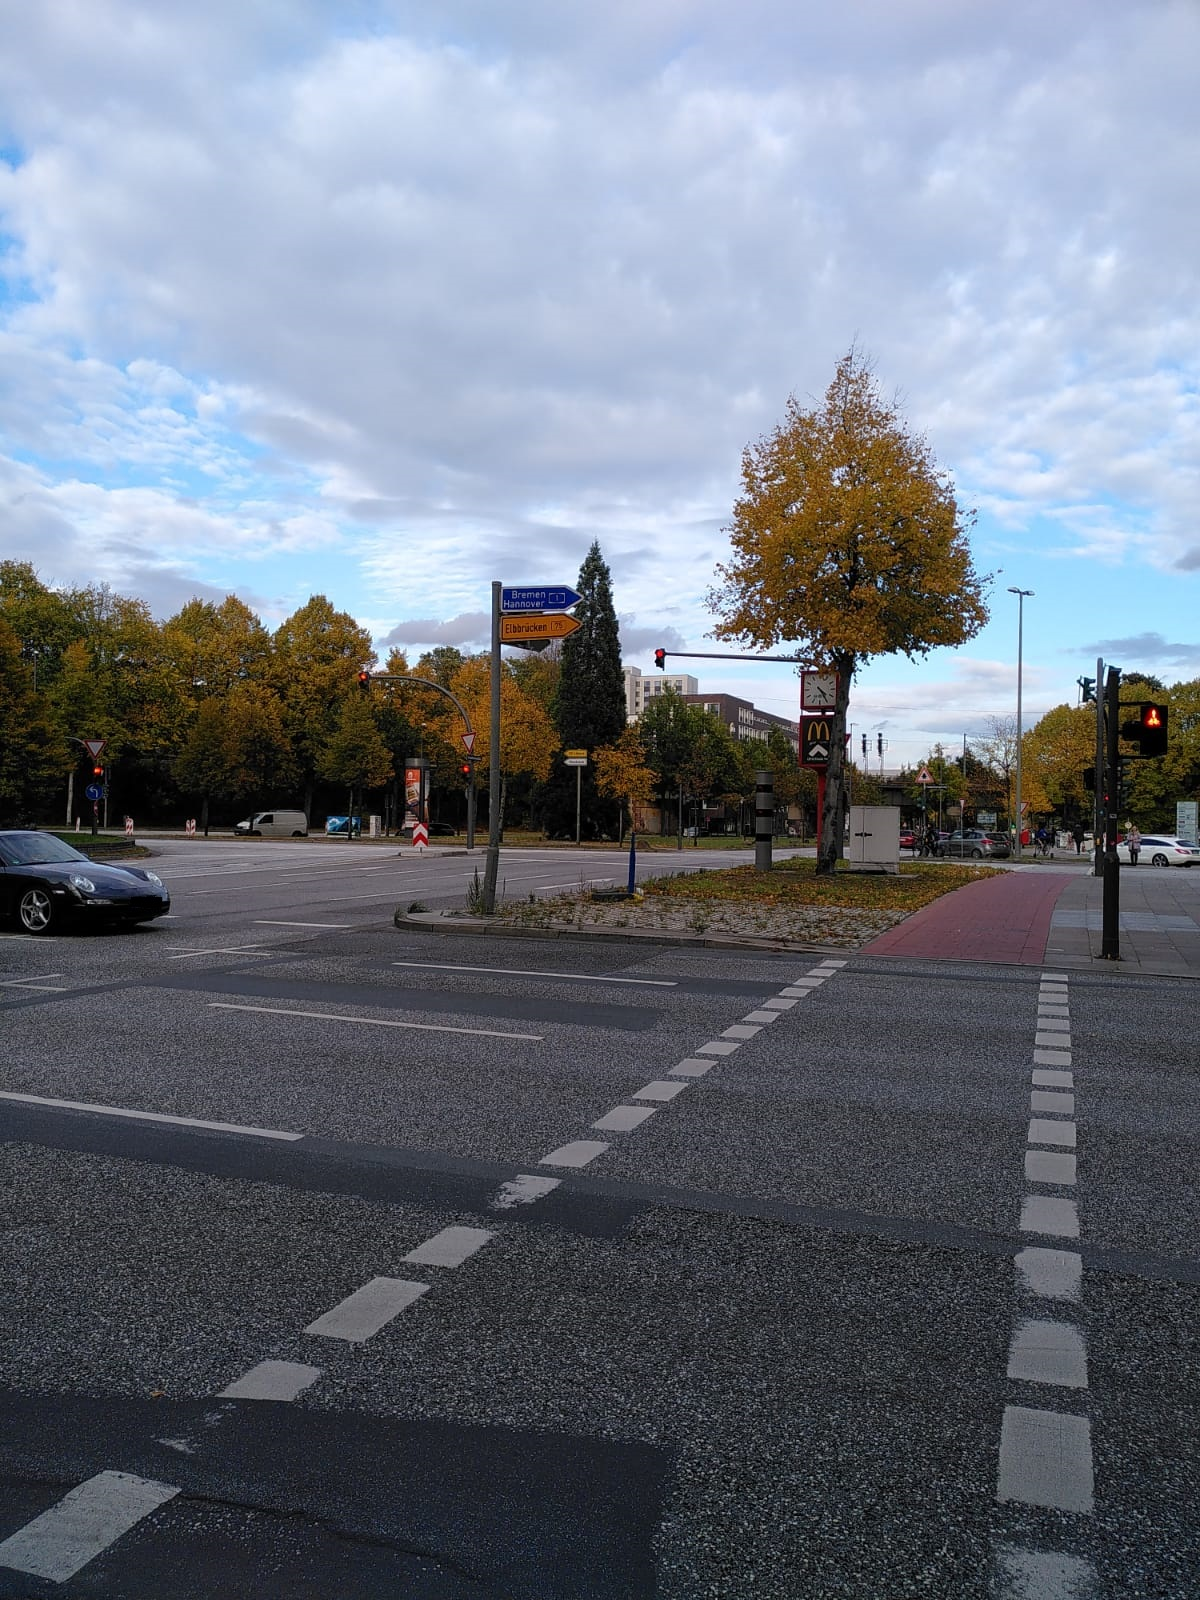
\includegraphics[scale=0.2]{Sections/Brainstorming/Blitzer.jpeg}
\caption{Blitzer Anckelmannsplatz}
\label{fig:Blitzer_Anckelmannsplatz}
\end{figure}

\begin{figure}[h]
\centering
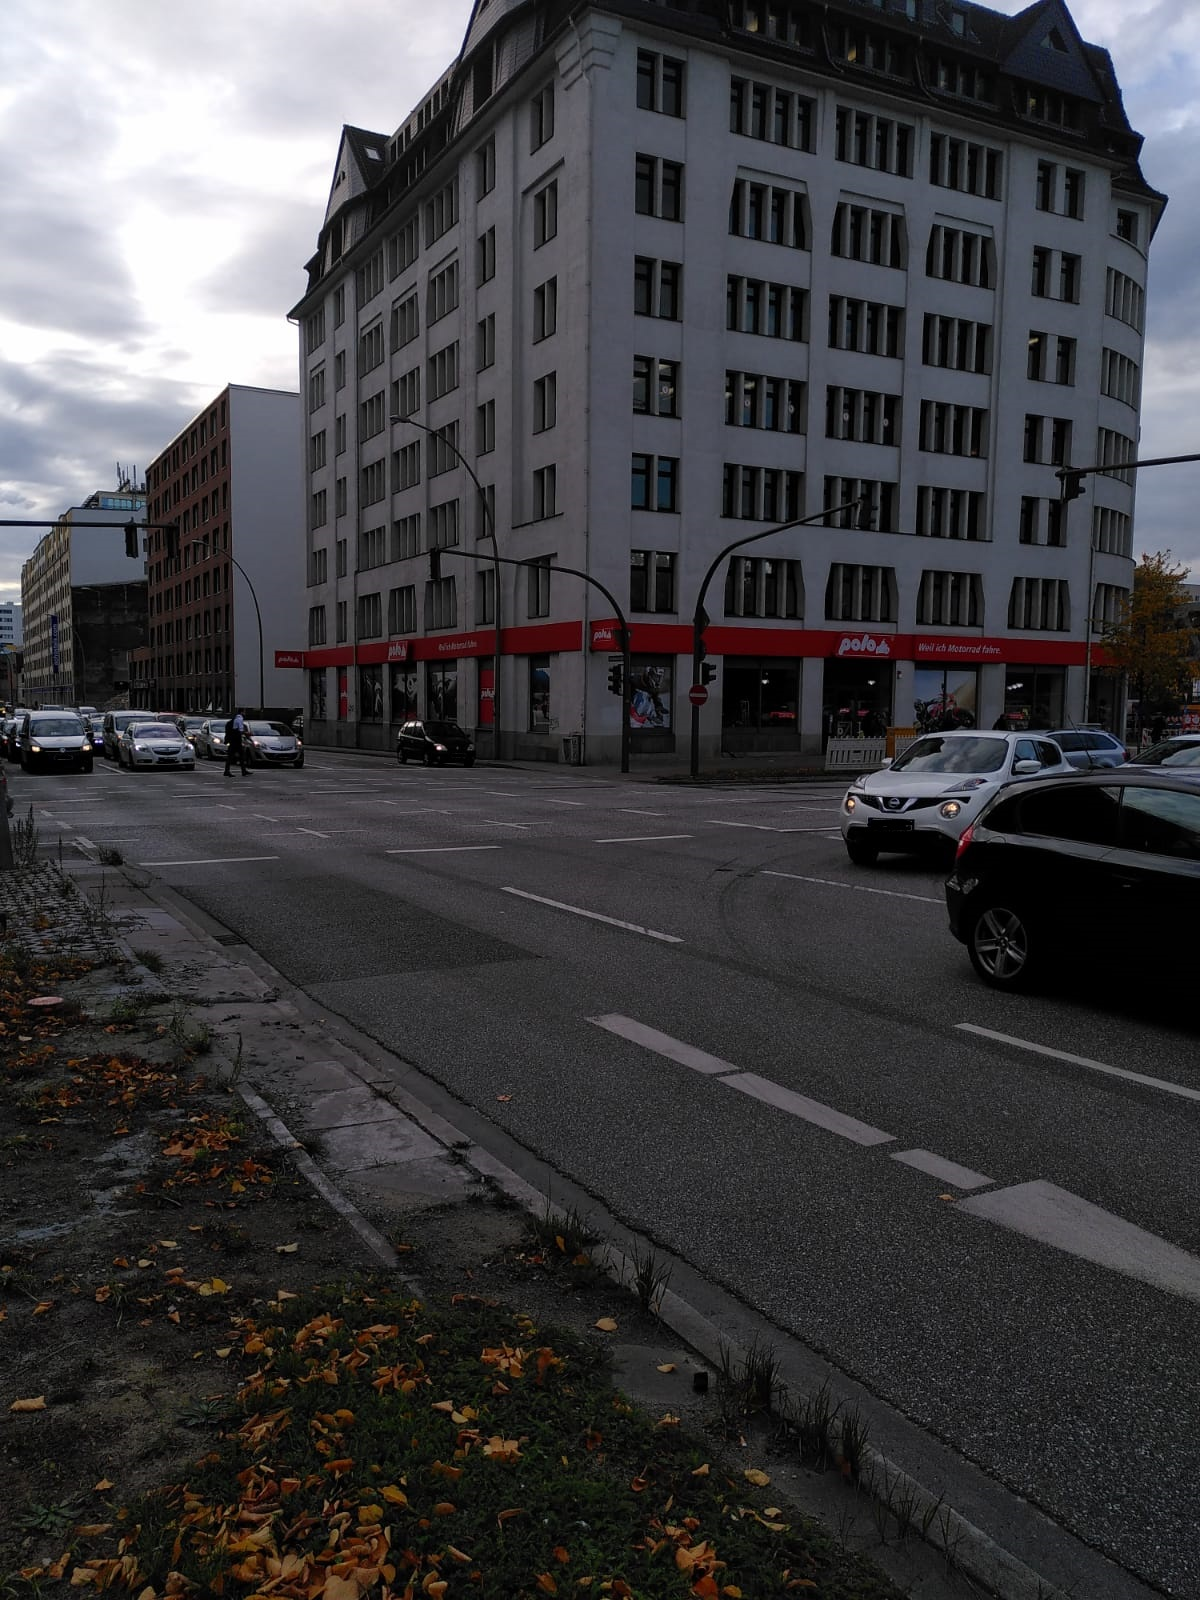
\includegraphics[scale=0.2]{Sections/Brainstorming/Blickwinkel_Blitzer_2.jpeg}
\caption{Blitzer Blickwinkel}
\label{fig:Blitzer_Blickwinkel}
\end{figure}

\newpage

\begin{figure}[h]
\centering
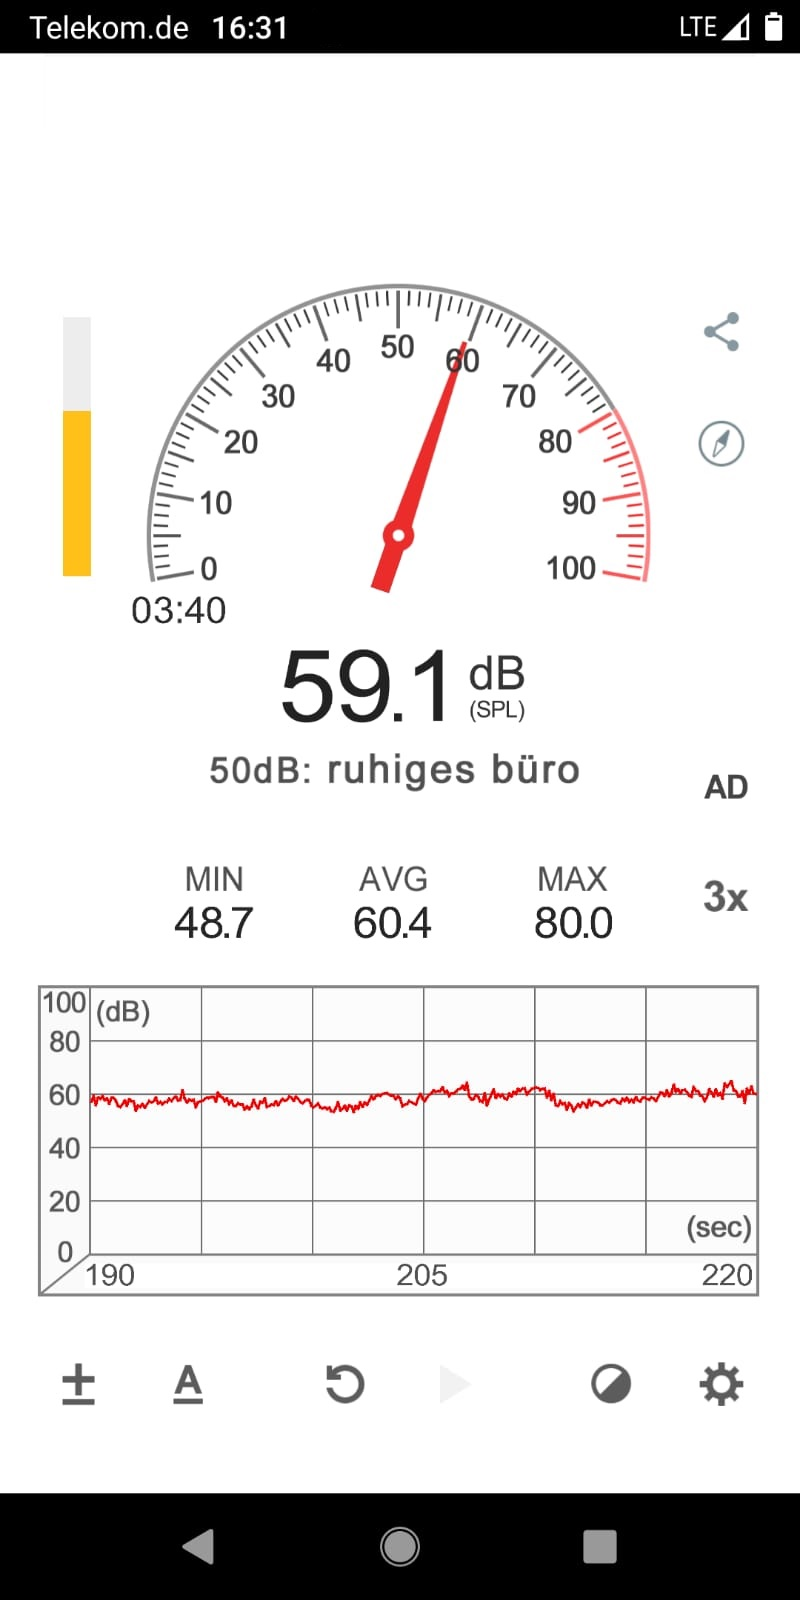
\includegraphics[scale=0.15]{Sections/Brainstorming/Pegelmessung_Anckelmannsplatz_am_Blitzer_Nachmittag.jpeg}
\caption{Schallmessung}
\label{fig:Schallmessung}
\end{figure}

Bild \ref{fig:Blitzer_Anckelmannsplatz} und \ref{fig:Blitzer_Blickwinkel} zeigen den oben genannten Blitzer, sowie den anzunehmenden Blinkwinkel. Öffnungswinkel des Detectors müssen noch erörtert werden. \\
\noindent Bild \ref{fig:Schallmessung} zeigt eine Schallmessung an einem gewöhnlichen Donnerstagnachmittag auf dem Anckelmannsplatz Höhe des Blitzers als Referenz des Pegelwertes.

\newpage

%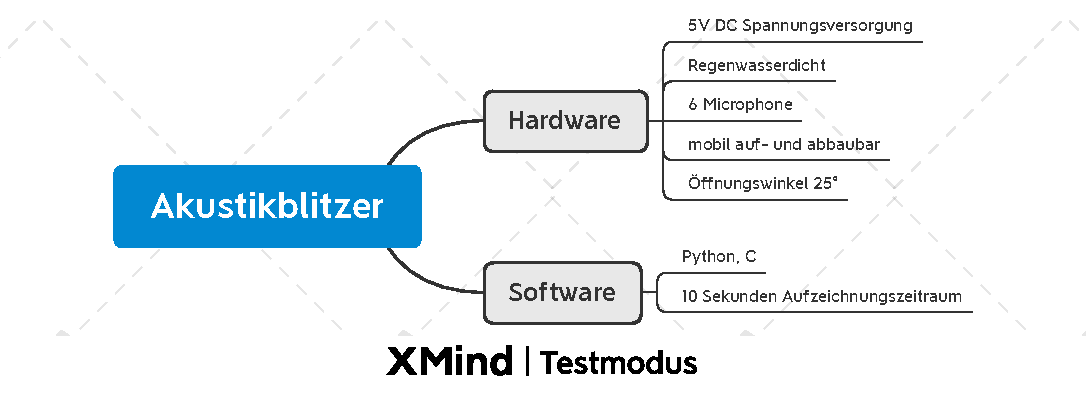
\includepdf[pages=-]{Sections/Brainstorming/2020-10-15_Brainstorming}

\newpage

\section{Meeting 22. 10. 2020}

Ort: Zoom-Online-Meeting
\newline
Zeit: 13:00 Uhr
\newline
Meeting-ID: 951 5710 6731
\newline
Kenncode: 179320
\newline
Protokollant: 
\newline
Vorläufige Themenauswahl:
\begin{itemize}
\item Ihre (unsere) Fragen
\item Zeitplanung
\item HW, SW
\item Verteilung der Aufgaben
\item weiteres:
\end{itemize}

\vspace{2cm}
\noindent
unsere Fragen:
\begin{enumerate}
\item Soll die Datenauswertung zeitgleich mit der Aufnahme erfolgen? \hfill $\Box$ Ja\qquad $\Box$ Nein
\item Wird die Berechnung intern auf dem Paspberry Pi ausgeführt? \hfill $\Box$ Ja\qquad $\Box$ Nein
\item Bekommen wir die Dokumentation und den Source Code des Schussdetektors heute noch? \hfill $\Box$ Ja\qquad $\Box$ Nein
\item Welche Art von Kamera soll in diesem System verwendet werden?
\item Welche Brennweite/ Öffnungswinkel ist gefordert?
\item Wie wird die Dämpfung trotz hoher IP Schutzklasse umgangen?
\item Mit welcher maximalen Fahrgeschwindigkeit muss das System zurechtkommen?
\item Ist ein 24h Betrieb gefordert? \hfill $\Box$ Ja\qquad $\Box$ Nein
\item Ab welchem Lautstärkepegel soll das System anschlagen?
\item Wie viele Fahrzeuge sollen simultan erfasst werden?
\item Wie viele Fahrspuren soll ein System überwachen?
\item Welche Wetter- und Temperaturverhältnisse soll das System vertragen können?
\item Soll das System erweiterbar sein? \hfill $\Box$ Ja\qquad $\Box$ Nein
\item Soll das System Redundanzen besitzen? \hfill $\Box$ Ja\qquad $\Box$ Nein
\item Soll das System mobil ausgelegt werden? \hfill $\Box$ Ja\qquad $\Box$ Nein
\item Nach welchen Umwelt und Recycling Standards arbeiten wir?
\item In welchem Bereich liegen die Messtoleranzen?
\item Welche Fehlerwahrscheinlichkeit ist akzeptabel?
\item Soll eine Fernwartung / ein Fernzugriff möglich sein? \hfill $\Box$ Ja\qquad $\Box$ Nein
\item Mit welcher Messfrequenz wird das System arbeiten?
\item Muss bei der Entwicklung auf Servicemaßnahmen geachtet werden? \hfill $\Box$ Ja\qquad $\Box$ Nein
\item Welche Rahmenbedingungen gelten für die Dokumentation?
\item Welche Möglichkeiten haben wir in der Werkstatt?
\end{enumerate}
\newpage

\section{Anforderungsanalyse}

\subsection{Lastenheft}

Es soll ein Prototyp für die Erkennung und Lokalisierung eines Kraftfahrzeuges mit (zu) hohen Lärmemissionen entwickelt werden. Dabei sollen innerorts bis \SI{50}{km/h} mindestens drei Fahrspuren, mit einer Option auf zwei weitere, abgedeckt werden. Der Detektor soll so konstruiert werden, dass er problemlos von einer einzelnen Person in einem handelsüblichen Rucksack verstaut und transportiert werden kann. Die mindestens verfügbare Einsatzdauer soll eine halbe Stunde betragen. Die im Einsatz erfassten Daten sollen innerhalb von zwei Sekunden an Peripheriegeräte gesendet werden, um dort von dem Benutzer kontrolliert werden zu können. Der Benutzer kann sich in einem Aktionsradius von maximal \SI{30}{m} befinden und soll die Möglichkeit der Fernwartung haben. Die Messtoleranz des Prototypen soll im Bereich von \SI{0,5}{m} und \SI{1}{m} liegen. Eine Fehlerwahrscheinlichkeit von 99\% soll erreicht werden. (\color{red}Den letzten Punkt bitte nochmal überdenken - Sinnprüfung\color{black}) Die Messung soll mit einer Messfrequenz von \SI{48}{kHz} bei 24 Bit durchgeführt werden.

\section{Pflichtenheft}

Bei der Erstellung des Pflichtenhefts wurde, basierend auf dem Lastenheft des Traffic-Noise--Detectors, auf die individuellen Forderungen des Auftraggebers eingegangen. Die daraus entstandenen Umsetzungen sind aus der folgenden Tabelle zu entnehmen:

\begin{center}
\begin{tabular}{|p{2cm}|p{6cm}|p{6cm}|}
\hline
\textbf{Ifd.-Nr} & \textbf{Anforderungen gemäß Lastenheft:} & \textbf{Umsetzung im Pflichtenheft:}\\
\hline
1 & Überwachung von drei Fahrspuren & Mit Hilfe von sechs Mikrophonen, welche durch den Auftraggeber bereitgestellt werden.\\
\hline
2 & Angemessenes Gewicht & Benötigte Halterungen/ Vorrichtungen werden bevorzugt mittels eines 3D-Druckverfahrens hergestellt, um so das Gewicht zu senken. \hfill\\
\hline
3 & Verstaubar in einem Rucksack & Ein entsprechendes Gehäuse wird durch den Auftraggeber zur Verfügung gestellt. \\
\hline
4 & Leicht aufbaubar & Als Unterbau wird ein Stativ aus dem Fotografie Bereich verwendet. Dieses verfügt bereits über eine passende Aufnahme für den Prototypen.\\
\hline
5 & Einsatzdauer > 0.5 Stunden & Die Energieversorgung wird mittels Akkumulatoren sichergestellt \\
\hline
6 & Übertragung der erfassten Daten in einem Aktionsradius von \SI{30}{m} & WLAN Netz \\
\hline
7 & Betreiben einer Fernwartung & WLAN Netz\\
\hline
8 & Messtoleranz im Bereich \SI{0,5}{m} und \SI{1}{m} & \\
\hline
9 & Fehlerwahrscheinlichkeit von 99\% & \\
\hline
10 & Die Messfrequenz soll \SI{48}{kHz} bei 24 Bit betragen \hfill & Das System wird entsprechend eingestellt \hfill \\
\hline
11 &&\\
\hline
12 &&\\
\hline
13 &&\\
\hline
14 &&\\
\hline
&&\\
\hline
&&\\
\hline
\end{tabular}
\end{center}

\section{Konstruktion des Aufbaus}

Für ein ressourcenschonendes Arbeiten ist es von großer Bedeutung neben den Methoden der Produktentwicklung auch diejenigen Materialien zu verwenden, die ohnehin schon vorrätig sind. In den entsprechenden Abschnitten wird noch näher drauf eingegangen. Zu bemerken sei aber noch, dass eine Verwendung der verfügbaren Materialien nicht immer die beste Option ist.

\subsection{Basisstativ}

In dem Labor \glqq Urban Mobility Lab\grqq\ liegt bereits das Fotostativ Manfrotto 055 bereit und kann verwendet werden. Herausfordernd kommt aber hinzu, dass sich ein 1/4\grqq\ Gewinde auf der Montageplatte befindet. Die folgenden Möglichkeiten zum Umgang mit dem Gewinde wurden diskutiert:

\begin{itemize}
	\item Nutenstein mit 1/4\grqq\ Innengewinde
	\item Adapterplatte zwischen Montageplatte und Trägerprofil
	\item Tausch der 1/4\grqq\ Schraube durch eine Schraube mit M4 Außengewinde
	\item Tausch des Stativs
\end{itemize}

Nach einer Anfrage bei item Industrietechnik GmbH nach Nutensteinen mit entsprechendem 1/4\grqq\ Innengewinde, war bekannt, dass sich derartige Produkte auf dem Markt nicht ohne Weiteres besorgen lassen.

Der Tausch des Stativs durch ein alternatives, ebenfalls zur Verfügung stehende, wurde ausgeschlossen, da die Dimensionen des Stativs eindeutig zu massiv sind und der Anforderung einer leichten Transportierbarkeit im Wege stehen.

Eine Adapterplatte aus einem Aluminium-Flachprofil wurde ausgeschlossen, da nach einer Untersuchung des Fotostativs sich herauskristallisiert hat, dass die eingebaute UNC Schraube einfach durch eine M4 Schraube getauscht werden kann.

\subsection{Mikrofongehäuse}

Dadurch, dass die zum Einsatz kommenden Mikrofone fertig auf einer Platine (\autoref{fig:Mikrofonplatine}) verbaut sind, aber damit nicht gegen Regenwasser geschützt sind, mussten im Entwicklungsprozess Gehäuse für die Mikrofone konstruiert und 3D-gedruckt werden. Nach sehr kurzer Diskussion war beschlossen, dass mittels CAD ein Gehäuse konstruiert und im vorhandenen 3D-Drucker gefertigt werden sollen (\autoref{fig:Mikrofongehäuse}).

\begin{figure}[h]
	\begin{center}
		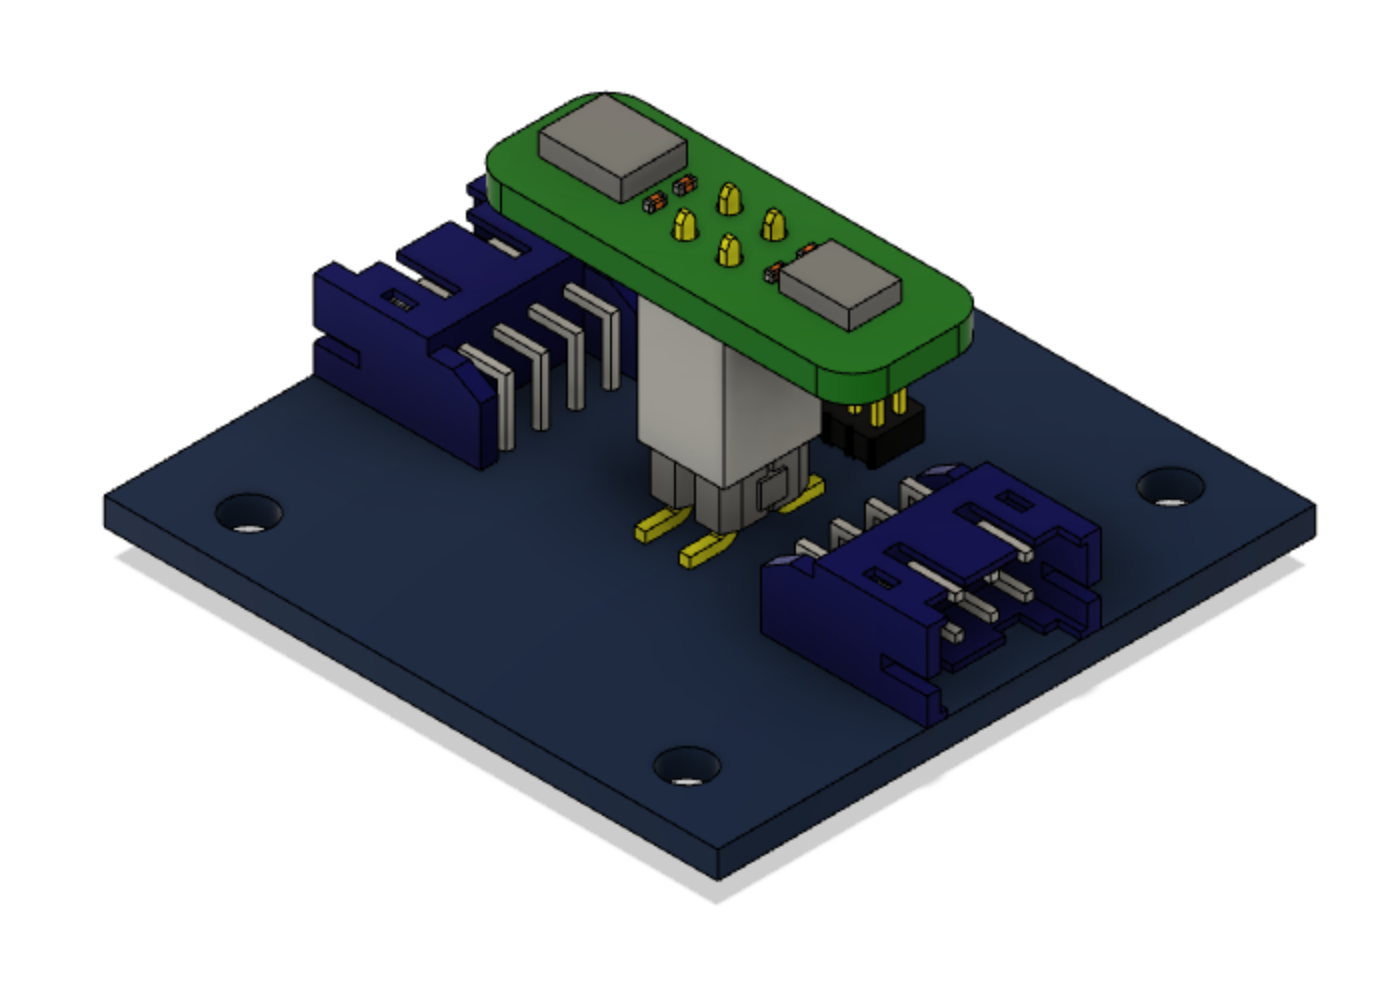
\includegraphics[scale=0.25]{Sections/Konstruktion_des_Aufbaus/Mikrofonplatine}
	\end{center}
	\caption{Mikrofonplatine}
	\label{fig:Mikrofonplatine}
\end{figure}

\newpage

\begin{figure}[h]
	\begin{center}
		\includegraphics[scale=0.25]{Sections/Konstruktion_des_Aufbaus/Mikrofongehäuse}
	\end{center}
	\caption{Mikrofongehäuse}
	\label{fig:Mikrofongehäuse}
\end{figure}

In der ersten Version dieser Gehäuse (\autoref{fig:Mikrofongehäuse_V_0.1}) soll die Mikrofonplatine über Stifte an Position gehalten und der Gehäusedeckel im Anschluss durch einen Längspressverband mit dem Gehäuseboden verbunden werden.

\begin{figure}[h]
	\begin{center}
		\includegraphics[scale=0.25]{Sections/Konstruktion_des_Aufbaus/Mikrofongehäuse_V_0.1}
	\end{center}
	\caption{Mikrofongehäuse V 0.1}
	\label{fig:Mikrofongehäuse_V_0.1}
\end{figure}


Nach dem Druck der sechs Gehäuse stellte sich heraus, dass:

\begin{enumerate}
	\item die gedruckten Stifte nicht maßhaltig sind
	\item die Löcher im Deckel nicht maßhaltig sind
	\item viele druckbedingte Fäden an den Teilen beseitigt werden müssen
\end{enumerate}

An der gedruckten Geometrie lässt sich im Nachgang nicht mehr viel bearbeiten, lediglich die Hülsen im Gehäusedeckel können aufgebohrt werden. Die Erfahrung hat aber gezeigt, dass das verwendete Filament vor allem an den Kontaktflächen der einzelnen Layer zu porös ist und beim Aufbohren sehr schnell bricht. Alle Gehäuse wurden entsorgt.

\newpage

\begin{figure}[h]
	\begin{center}
		\includegraphics[scale=0.2]{Sections/Konstruktion_des_Aufbaus/Mikrofongehäuse_V_0.2}
	\end{center}
	\caption{Mikrofongehäuse V 0.2}
	\label{fig:Mikrofongehäuse_V_0.2}
\end{figure}

Für die zweite Version (\autoref{fig:Mikrofongehäuse_V_0.2}) der Gehäuse wurden die Stifte im Unterteil und die Hülsen im Deckel entfernt. Im Unterteil sind nun Sechskantaufnahmen für vier M2.5 Muttern und im Deckel Durchgangslöcher für entsprechend Lange Zylinderkopfschrauben. Durch Einpressen und Verkleben werden die Muttern in Position gehalten.

Die Mikrofonplatine wird auf die Flächen auf die Flächen oberhalb der Mutter aufgelegt und das Gehäuse durch Anziehen der vier Schrauben verschlossen. Nach dem Druck eines neuen Prototyps wurde die Brauchbarkeit analysiert und das Gehäuse für die Massenproduktion freigegeben. Nachteilig ist, dass mit ausreichend großer Zugkraft die Gehäusedeckel trotz Verschraubung geöffnet werden können, zudem wirken die vier Schrauben etwas überdimensioniert. In einer zweiten Überarbeitung sollten diese beiden Punkte beachtet werden.

\subsection{Unterbringung der Steuereinheit}

Für den Raspberry Pi 4, die Raspicam v2.1 und die Powerbank Powerbank PLUS MacBook 20.100 mAh Space Grey sollte eine vorhandene wasserfeste Installationsbox verwendet werden. Das Hauptproblem dabei war, die zu Powerbank in der Box zu plazieren, daher wurde sich entschlossen, eine neue Installationsbox zu bestellen (Hammond Manufacturing 1555VAL2GY). Für die sichere Positionierung aller Bauteile wird wieder auf die 3D-Druck-Technologie zurückgegriffen und ein Innenleben konstruiert.

Nach der ersten Konstruktion stellte sich heraus, dass die neu besorgte Installationsbox zu niedrig für das Innenleben ist und die USB Kontakte des Rapsberry Pi 4 durch den Deckel stoßen (\autoref{fig:Schnitt_Installationsbox_V_0.1}). In einem Teamreview wurde eine mögliche Lösung entwickelt, bei der der Raspberry Pi 4 sowohl \ang{180} um die Längs-, als auch \ang{90} im Uhrzeigersinn um die Querachse gedreht, eingebaut werden sollte. Nach der Neukostruktion und der Ergänzung einer Stützkonstruktion für den Raspberry Pi 4, war es möglich in der Installationsbox alle Bauteile zu platzieren, ohne eine erneute Neuanschaffung zu tätigen. (\autoref{fig:Schnitt_Installationsbox_V_0.2})

\begin{figure}[h]
	\begin{center}
		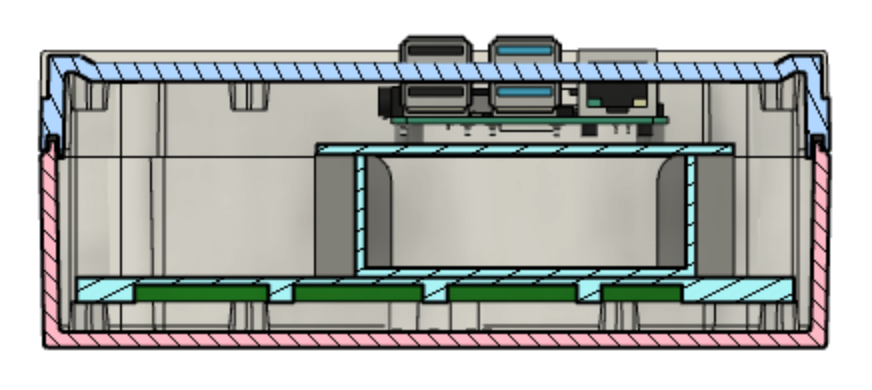
\includegraphics[scale=0.25]{Sections/Konstruktion_des_Aufbaus/Schnitt_Installationsbox_V_0.1}
	\end{center}
	\caption{Schnitt Installationsbox V 0.1}
	\label{fig:Schnitt_Installationsbox_V_0.1}
\end{figure}

Bei der Finalisierung des Aufbaus ist nochmals aufgefallen, wie maßungenau der 3D-Drucker arbeitet, so dass die Akkuwanne längs aufgesägt und die Löcher für die Schrauben aufgeweitet werden mussten.

\begin{figure}[h]
	\begin{center}
		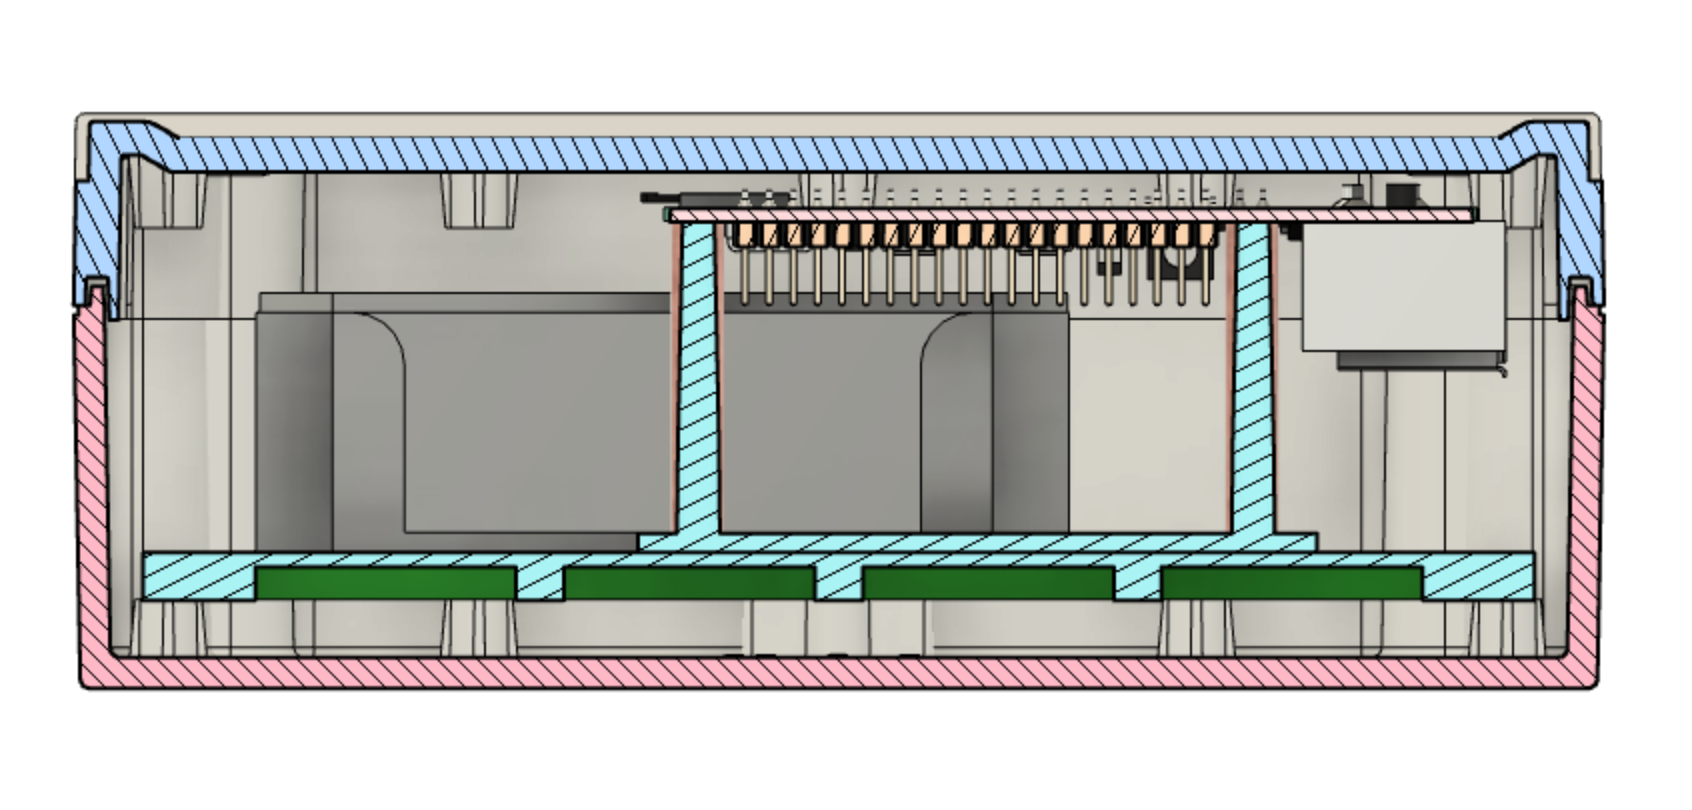
\includegraphics[scale=0.28]{Sections/Konstruktion_des_Aufbaus/Schnitt_Installationsbox_V_0.2}
	\end{center}
	\caption{Schnitt Installationsbox V 0.2}
	\label{fig:Schnitt_Installationsbox_V_0.2}
\end{figure}

\subsection{Positionierung der Baugruppen entlang eines Arrays}

Um die Mikrofone entlang einer Linie positionieren zu können, wurde ein \SI{1,1}{m} langes vorhandenes item-Profil 6 30x30 eingesetzt, auf dem die Gehäuse der Mikrofone mit Nutensteinen in definiertem Abstand montiert werden können. Dazu wurden am Mikrofongehäuse jeweils rechts und links zwei Befestigungspunkte für M4 Schrauben designt. Als Gegenstück werden wieder Nutensteine eingesetzt.

Das Profil an sich wird, wie oben beschrieben, auch mittels eines Nutensteins auf dem Stativ befestigt. Die Installationsbox wird ebenfalls mit Nutensteinen mittig am Profil befestigt.

\newpage

\end{document}